% ****** Start of file apssamp.tex ******
%
%   This file is part of the APS files in the REVTeX 4.1 distribution.
%   Version 4.1r of REVTeX, August 2010
%
%   Copyright (c) 2009, 2010 The American Physical Society.
%
%   See the REVTeX 4 README file for restrictions and more information.
%
% TeX'ing this file requires that you have AMS-LaTeX 2.0 installed
% as well as the rest of the prerequisites for REVTeX 4.1
%
% See the REVTeX 4 README file
% It also requires running BibTeX. The commands are as follows:
%
%  1)  latex apssamp.tex
%  2)  bibtex apssamp
%  3)  latex apssamp.tex
%  4)  latex apssamp.tex

%Set document type
\documentclass[
  reprint,
  amsmath,amssymb,
  aps
]{revtex4-1}


%Import packages similar to importing libraries in python.
\usepackage{float}
\usepackage{physics}

\usepackage{graphicx} %Include figure files
\graphicspath{ {figures/} } % Figure file location
\usepackage{subcaption}

\usepackage{dcolumn}% Align table columns on decimal point
\usepackage{bm}% bold math

\usepackage{bookmark}

%Import this last. Allows clickable figures, equations, and links.
\usepackage{hyperref} % add hypertext capabilities
\hypersetup{
    colorlinks = true,
    linkcolor = black,
    filecolor = magenta,      
    urlcolor = cyan,
    citecolor = blue,
    }




%Latex does \begin{...} and \end{...}
\begin{document}

\title{A Overview of Quantum Tunneling in MOSFETs\\and its Contributions to MOSFET Scaling}


\author{Lawrence Liu}
\affiliation{Department of Electrical and Computer Engineering, University of California\textbf{--}Los Angeles, Los Angeles, California 90095, USA}

%\date{\today}% It is always \today, today,
             %  but any date may be explicitly specified

% \begin{abstract}
% This template is used for Physical Review Letter (PRL) submissions. Different journals have different formatting requirements, such as the Journal of High Energy Physics (JHEP). If you're familiar with LaTeX, then you can use a different template if you'd like. Otherwise, I've attached some example code that will walk you through some of the basics of creating sections, subsections, and referencing figures and equations. The example code should be enough to get you started, but LaTeX can do so much more. I encourage you to explore online.
% \end{abstract}

%bookmarksetup creates bookmarks at root level.
%Otherwise the title is one collapsible bookmark
\maketitle
\bookmarksetup{startatroot}

%Table of contents command
%\tableofcontents

\section{\label{sec:level1}Introduction}
Metal Oxide Semiconductor Field Effect Transistors (MOSFETs) are the most common type of transistor used in modern electronics. Let us start 
by briefly discussing the basic operation of a MOSFETs and a common application of MOSFETs in Complemetary Metal Oxide Semiconductor (CMOS) logic gates.
\subsection*{Basic MOSFET Structure}
The MOSFET is based around a Metal Oxide Semiconductor (MOS) capacitor. Historically this 
was a gate made out of a metal plate on top of a semiconductor substrate, which was separated by an insulating layer of oxide, however modern 
MOSFETs use a polysilicon gate instead of a metal gate.\\\\
Now to make a MOSFET we add a source and drain silicon regions to the silicon substrate. The source and drain regions are doped with impurities to
be the opposite type to that of the base silicon substrate. For example, if the base silicon substrate is p-type, then the source and drain regions
are n-type, and vice versa. We call the MOSFET with n-type source and drain regions an nMOSFET, and the MOSFET with p-type source and drain regions. We have 
drawn both an nMOSFET and a pMOSFET in Figure \ref{fig:mosfet} along with their respective circuit symbols.\\\\
\begin{figure}[H]
    \centering
    \begin{subfigure}[b]{0.45\textwidth}
        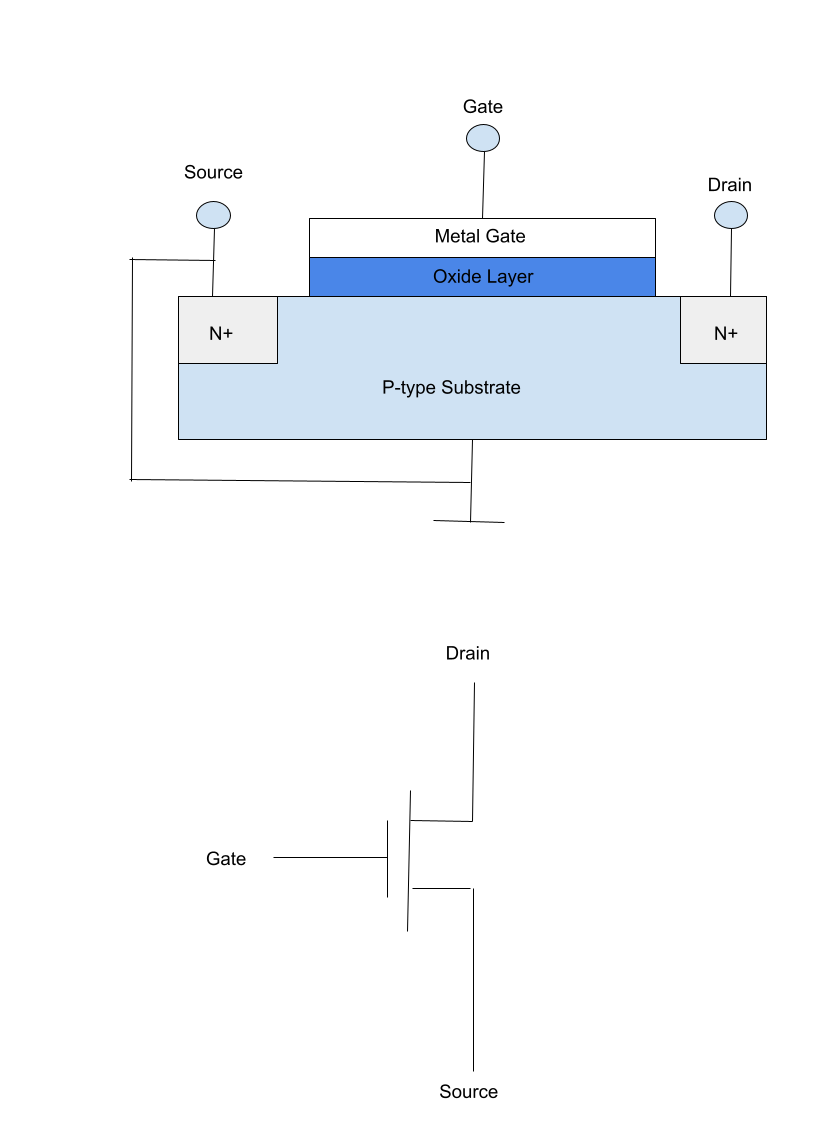
\includegraphics[width=\linewidth]{nmosfet.png}
        \caption{nMOSFET}
        \label{fig:nmosfet}
    \end{subfigure}
    \begin{subfigure}[b]{0.45\textwidth}
        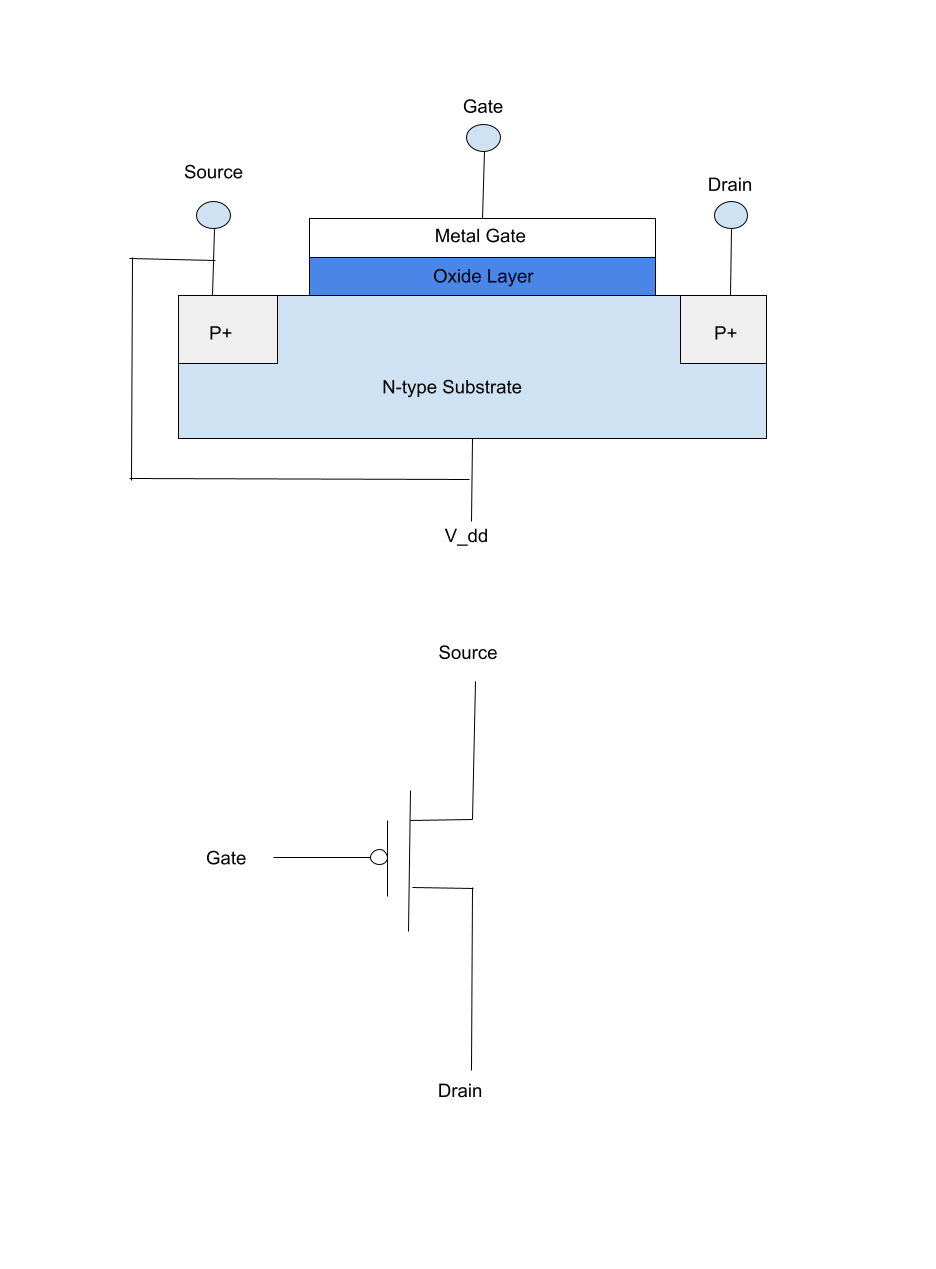
\includegraphics[width=\linewidth]{pmosfet.png}
        \caption{pMOSFET}
        \label{fig:pmosfet}
    \end{subfigure}
    \caption{MOSFETs and their circuit symbols.}
    \label{fig:mosfet}
\end{figure}
Let us define $V_{ds}$ as the voltage between the drain and source, and $V_{gs}$ as the voltage between the gate and source.
\subsection*{MOSFET Operation}
Now let us consider a the operation of a nMOSFET in a qualitative sense. If we apply a positive voltage to the gate, then 
the holes in the p-type substrate will be pushed away from the gate, or more accurately, the minority electrons will be drawn 
to the gate. If enough are drawn to the gate, then an inversion layer of n-type Silicon will form at the surface of the substrate since 
enough electrons will be present to become the majority carrier. This inversion layer will form a conductive channel between the source and drain, 
allowing current to flow between the source and drain. Therefore in a very rough sense, we can see that a MOSFET acts 
as a voltage controlled switch.\\\\
In a more rigorous sense, what happens is that the gate voltage "bends" the energy bands in the p-type substrate lower. 
Once these bands bend to the degree that near the surface of the substrate, the conduction band is closer to the 
Fermi level than the valence band, then the inversion layer will form. This threshold is given by 
\begin{equation}
    V_{T} = V_{FB} + 2\phi_{B} + \frac{Q_{SS}}{C_{OX}}
    \label{eq:threshold_nMOSFET}
\end{equation}
Where $V_{FB}$ is the flatband voltage, ie the difference in the work functions of the gate and the substrate, $\phi_{B}$ is the 
difference between the Fermi level and the intrinsic Fermi level divided by the electron charge, $Q_{SS}=\sqrt{2\epsilon_{s}qN_{a}(2\phi_{B})}$ where 
$N_a$ is the doping concentration of the substrate, and $C_{OX}$ is the capacitance of the oxide layer.\\\\
We can see that the opposite happens for a pMOSFET. If we apply a negative voltage to the gate, then since the electrons are pushed 
away and the holes are drawn to the gate, then an inversion layer of p-type Silicon will form at the surface of the substrate. Or 
from a bands perspective, the bands will be "bended" upwards to the degree that the valence band is closer to the Fermi level than the
conduction band. We have that this threshold is given by
\begin{equation}
    V_{T} = V_{FB} - 2\phi_{B} - \frac{2\epsilon_{s}qN_{d}(2\phi_{B})}{C_{OX}}
    \label{eq:threshold_pMOSFET}
\end{equation}
Where $N_d$ is the doping concentration of the substrate.\\\\
Thus when we a apply a voltage greater or less than the threshold voltage for the nMOSFET and pMOSFET respectively, then the inversion layer will form. We 
can view this layer as a effectively a resistor between the source and drain. However as we increase the current across the 
drain and the source $V_{DS}$, we will start to experience "pinch off" where the inversion layer will start to narrow. Once the 
voltage is high enough, the inversion layer will pinch off completely, and no longer connect the source and drain. This is 
depicted in Figure \ref{fig:mosfet pinch off}. This will cause the MOSFET to no longer act as a voltage controlled 
resistor between the source and drain, and instead act as a voltage controlled current source. We call this 
operation region the "saturation" region as opposed the "Ohmic" region where the MOSFET acts as a voltage controlled resistor.\\\\
\begin{figure}
    \centering
    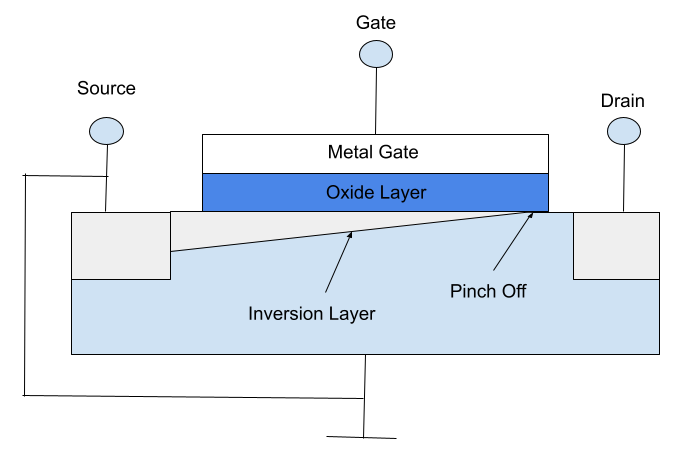
\includegraphics[width=0.5\linewidth]{mosfet_pinch_off.png}
    \caption{Pinch off in a MOSFET.}
    \label{fig:mosfet pinch off}
\end{figure}
The threshold for $V_{DS}$ at which the MOSFET enters the saturation region can be approximated by
\begin{equation}
    V_{DS,sat} = V_{GS} - V_{T}
\end{equation}
The current in the saturation region therefore can be approximated by
\begin{equation}
    I_{D,sat} = \frac{1}{2}C_{OX}\frac{W}{L}(V_{GS}-V_{T})^{2}
    \label{eq:mosfet saturation current}
\end{equation}
Where $W$ is the width of the MOSFET and $L$ is the length of the MOSFET.
\subsection*{Examples of MOSFET based circuits}
\subsubsection*{CMOS Inverter}
By connecting a pMOSFET and a nMOSFET in series, we can create a CMOS inverter. This is depicted in Figure \ref{fig:cmos inverter}.\\\\
\begin{figure}[H]
    \centering
    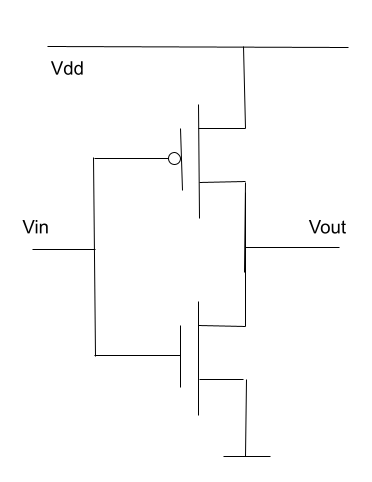
\includegraphics[width=0.5\linewidth]{cmos_inverter.png}
    \caption{CMOS inverter.}
    \label{fig:cmos inverter}
\end{figure}
To understand this circuit let us consider two cases when the input is "low" and when the input is "high". Let us assume that 
we have biased the circuit such that the threshold voltage of the nMOSFET is equal to the threshold voltage of the pMOSFET. Then in the 
case where the input is low, then the nMOSFET will be effectively an open circuit, and the pMOSFET will be effectively a closed circuit. Therefore the output will be high. 
Conversely, if the input is high, then the nMOSFET will be effectively a closed circuit, and the pMOSFET will be effectively an open circuit. Therefore the output will be low. Thus we can see that this circuit acts as an inverter.\\\\
\subsubsection*{CMOS NOR GATE}
We can make a NOR gate by connecting two nMOSFETs in parallel, this is depicted in Figure \ref{fig:cmos nor}.\\\\
\begin{figure}[H]
    \centering
    \includegraphics[width=0.5\linewidth]{cmos_nor.png}
    \caption{CMOS NOR gate.}
    \label{fig:cmos nor}
\end{figure}
As we can see, if any of the inputs are high, then there will be a connection between the output and ground. Thus the output will be low. Conversely, if all of the inputs are low, then there will be no connection between the output and ground. Thus the output will be high. 
Thus we can see that this circuit acts as a NOR gate. This is important because a NOR gate is algebraically complete, meaning that any boolean function can be implemented using only NOR gates.\\\\
\subsubsection*{Speed}
In our previous discussion about MOSFETs we neglected to include the parasitic capacitances that exist in the MOSFET when we 
view it from the source. These capacitances can come from the wires connecting the MOSFET, and the capacitance that is formed in the 
PN junction between the source and drain and the substrate. These capacitances resist changes in voltage, and thus slow down the 
MOSFET. We have that:
\begin{equation}
  \tau \propto \frac{C}{I_{on}}V_{DD}
\end{equation}
\section*{MOSFET Sizing}
Now armed with the knowledge of how MOSFETs work, let us examine how the size of a MOSFET can affect its performance, and why 
it is beneficial to have a smaller MOSFET. The most intuitive reason is that a smaller MOSFET will alow us to fit more MOSFETs
on a single chip, which allows for more digital circuits to be implemented on 
one chip, and thus driving down the cost per circuit.\\\\
Furthermore, by modifying other parameters of the MOSFET size, we
can also increase the speed and power efficiency of the MOSFET. 
Let us consider the capacitance of the Oxide layer of a MOSFET. We have that if the Oxide has a thickness of $t_{ox}$, 
an area of $A$, and a dielectric constant of $\epsilon_{ox}$, then the capacitance of the oxide layer is given by
\begin{equation}
  C_{ox} = \frac{\epsilon_{ox}A}{t_{ox}}
\end{equation}
Now if we consider a MOSFET with a thinner oxide layer $\alpha t_{ox}$ we 
have that the capacitance of the oxide layer is given by
\begin{equation}
  C_{ox} = \frac{\epsilon_{ox}A}{\alpha t_{ox}}
\end{equation}
Therefore we can see that the capacitance of the oxide layer is inversely proportional to the thickness of the oxide layer. Now if we return to 
equations (\ref{eq:threshold_nMOSFET}) and (\ref{eq:threshold_pMOSFET}), we can see that the threshold voltage is varies inversely proportional to the capacitance of the oxide layer. 
Thus a thinner oxide layer will have a lower threshold voltage. This is important because a lower threshold voltage means that the MOSFET will require less voltage, and therefore 
at a same current, will dissipate less power.\\\\
This will also affect the speed of the MOSFET by increasing the on current. We have that the on current given by 
equation (\ref{eq:mosfet saturation current}) is proportional to $(V_{GS}-V_{T})^{2}$. Therefore a lower threshold voltage will result in 
a higher on current. Now if we recall that the switch time of a MOSFET is proportional to $\frac{1}{I_{on}}$. Therefore 
a smaller threshold voltage will result in a faster switch time, or alternatively a lower power dissipation for the 
same switching time.\\\\
\subsection*{Issues with MOSFET Scaling}
Then what would stop us from making our MOSFETs smaller and smaller? Well, there will be several issues that will 
arise as we make our MOSFETs smaller. Of course the most obvious issue is that it will be harder to manufacture smaller MOSFETs. Furthermore, 
as we make our MOSFETs smaller, the behaviour of the MOSFET will be less dependent on the Classical Physics that the pervious 
equations were derived from. As an example, we will examine how scaling down the 
MOS capacitor will cause Quantum Tunneling to become a significant factor in the behaviour of the MOSFET. We will 
then examine how this will affect the behaviour of the MOSFET and how we can mitigate this effect.\\\\
\section*{Bardeen Tunneling Theory}
Let us start by briefly summarizing Bardeen Tunneling Theory. Let us consider a quantum mechanical system as depicted in 
Figure \ref{fig:bardeen tunneling} consisting of two potential wells separated by a barrier:\\\\
\begin{figure}[H]
    \centering
    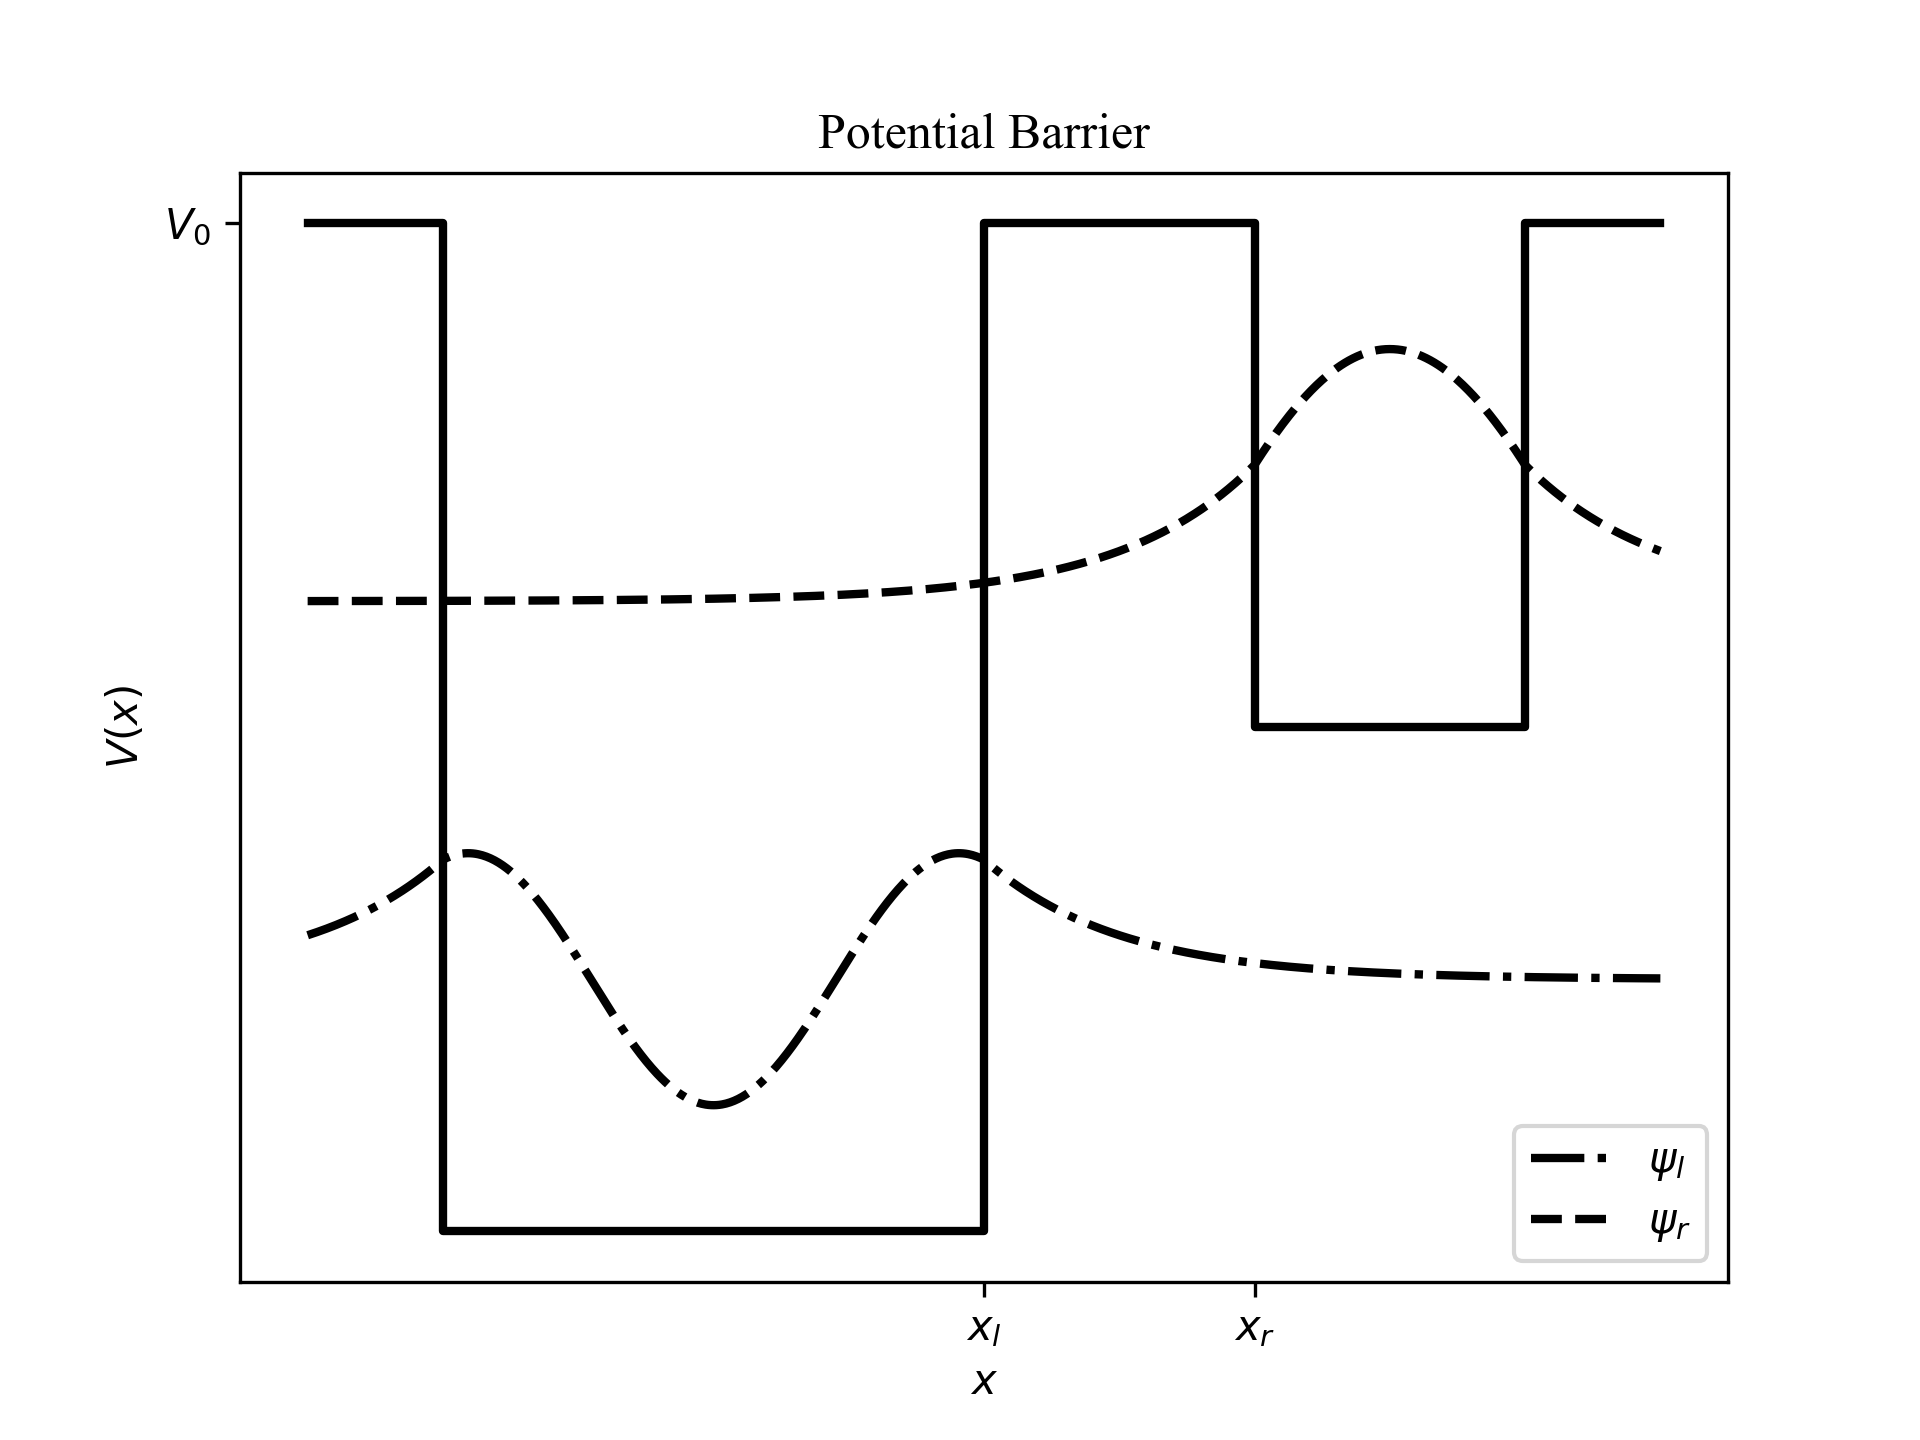
\includegraphics[width=0.5\linewidth]{bardeen_tunneling.png}
    \caption{Potential wells and wavefunctions.}
    \label{fig:bardeen tunneling}
\end{figure}
As we depicted, let us assume that both of these potential wells are symmetric around their own origins, and thus 
the potential outside the well is the same, which we defined in figure (\ref{fig: bardeen tunneling}) to be $V_0$. 
Then we have that the potential is given by
\begin{equation}
    V(x) = \begin{cases}
        V_l(x) & x < x_1\\
        V_r(x) & x \geq x_1
    \end{cases}
\end{equation}
Where $V_l(x)$ is the potential function for the left well, and $V_r(x)$ is the potential function for the right well, and 
$x_1$ is some arbitrary point $x_l<x_1<x_r$. We can see that we can express this as: 
\begin{equation}
    V(x) = V_l(x) - \Theta(x-x_1)(V_0-V_r(x))
\end{equation}
Where $\Theta(x)$ is the Heaviside step function. 
Therefore we can see that we can write the hamiltonian for this system as:
\begin{equation}
    H = \frac{p^2}{2m} + V_l(x) - \Theta(x-x_1)(V_0-V_r(x))
\end{equation}
We can see that if we define $H_l$ as the hamiltonian of a system consisting solely of the left well, and $H' = 
\theta(x-x_1)(V_0-V_r(x))$, then we can write the hamiltonian as:
\begin{equation}
    H = H_l + H'
\end{equation}
Therefore we can see the that the tunneling rate can be modeled by with Fermi's Golden Rule, with $H'$ as the perturbation that 
turns on at $t=0$. If we 
make the key assumption that the energy of the left well is approximately equal to the energy of the right well, ie 
$E_l \approx E_r =E$. We have that the transition rate is given by:
\begin{equation}
    \Gamma_{l\rightarrow r} = \frac{2\pi}{\hbar}\abs{\bra{r}H'\ket{l}}^2\rho(E)
\end{equation}
We have that the matrix element is given by:
\begin{equation}
    \bra{r}H'\ket{l} = \int_{-\infty}^{\infty}\psi_r^*(x)H'\psi_l(x)dx
\end{equation}
After doing some simplifications derived in the appendix, and with the assumption that $E_l \approx E_r =E$ we have that the matrix element is given by:
\begin{equation}
    \bra{r}H'\ket{l} = \frac{\hbar^2}{2m}\left(
        \psi_r^*\frac{d}{dx}\psi_l - \psi_l\frac{d}{dx}\psi_r^*
    \right)\Bigg|_{x=x_1}
\end{equation}
Which is the important result of Bardeen Tunneling Theory. 
\subsection*{Application to MOSFETs}
Now let us use it to try to approximate the gate source tunneling current 
of a MOSFET.





\bibliographystyle{abbrv}%Used BibTeX style is unsrt
\bibliography{references}

\end{document}